\providecommand{\main}{../../../..}
\documentclass[\main/dresen_thesis.tex]{subfiles}

\begin{document}
  \begin{figure}[!htbp]
    \centering
    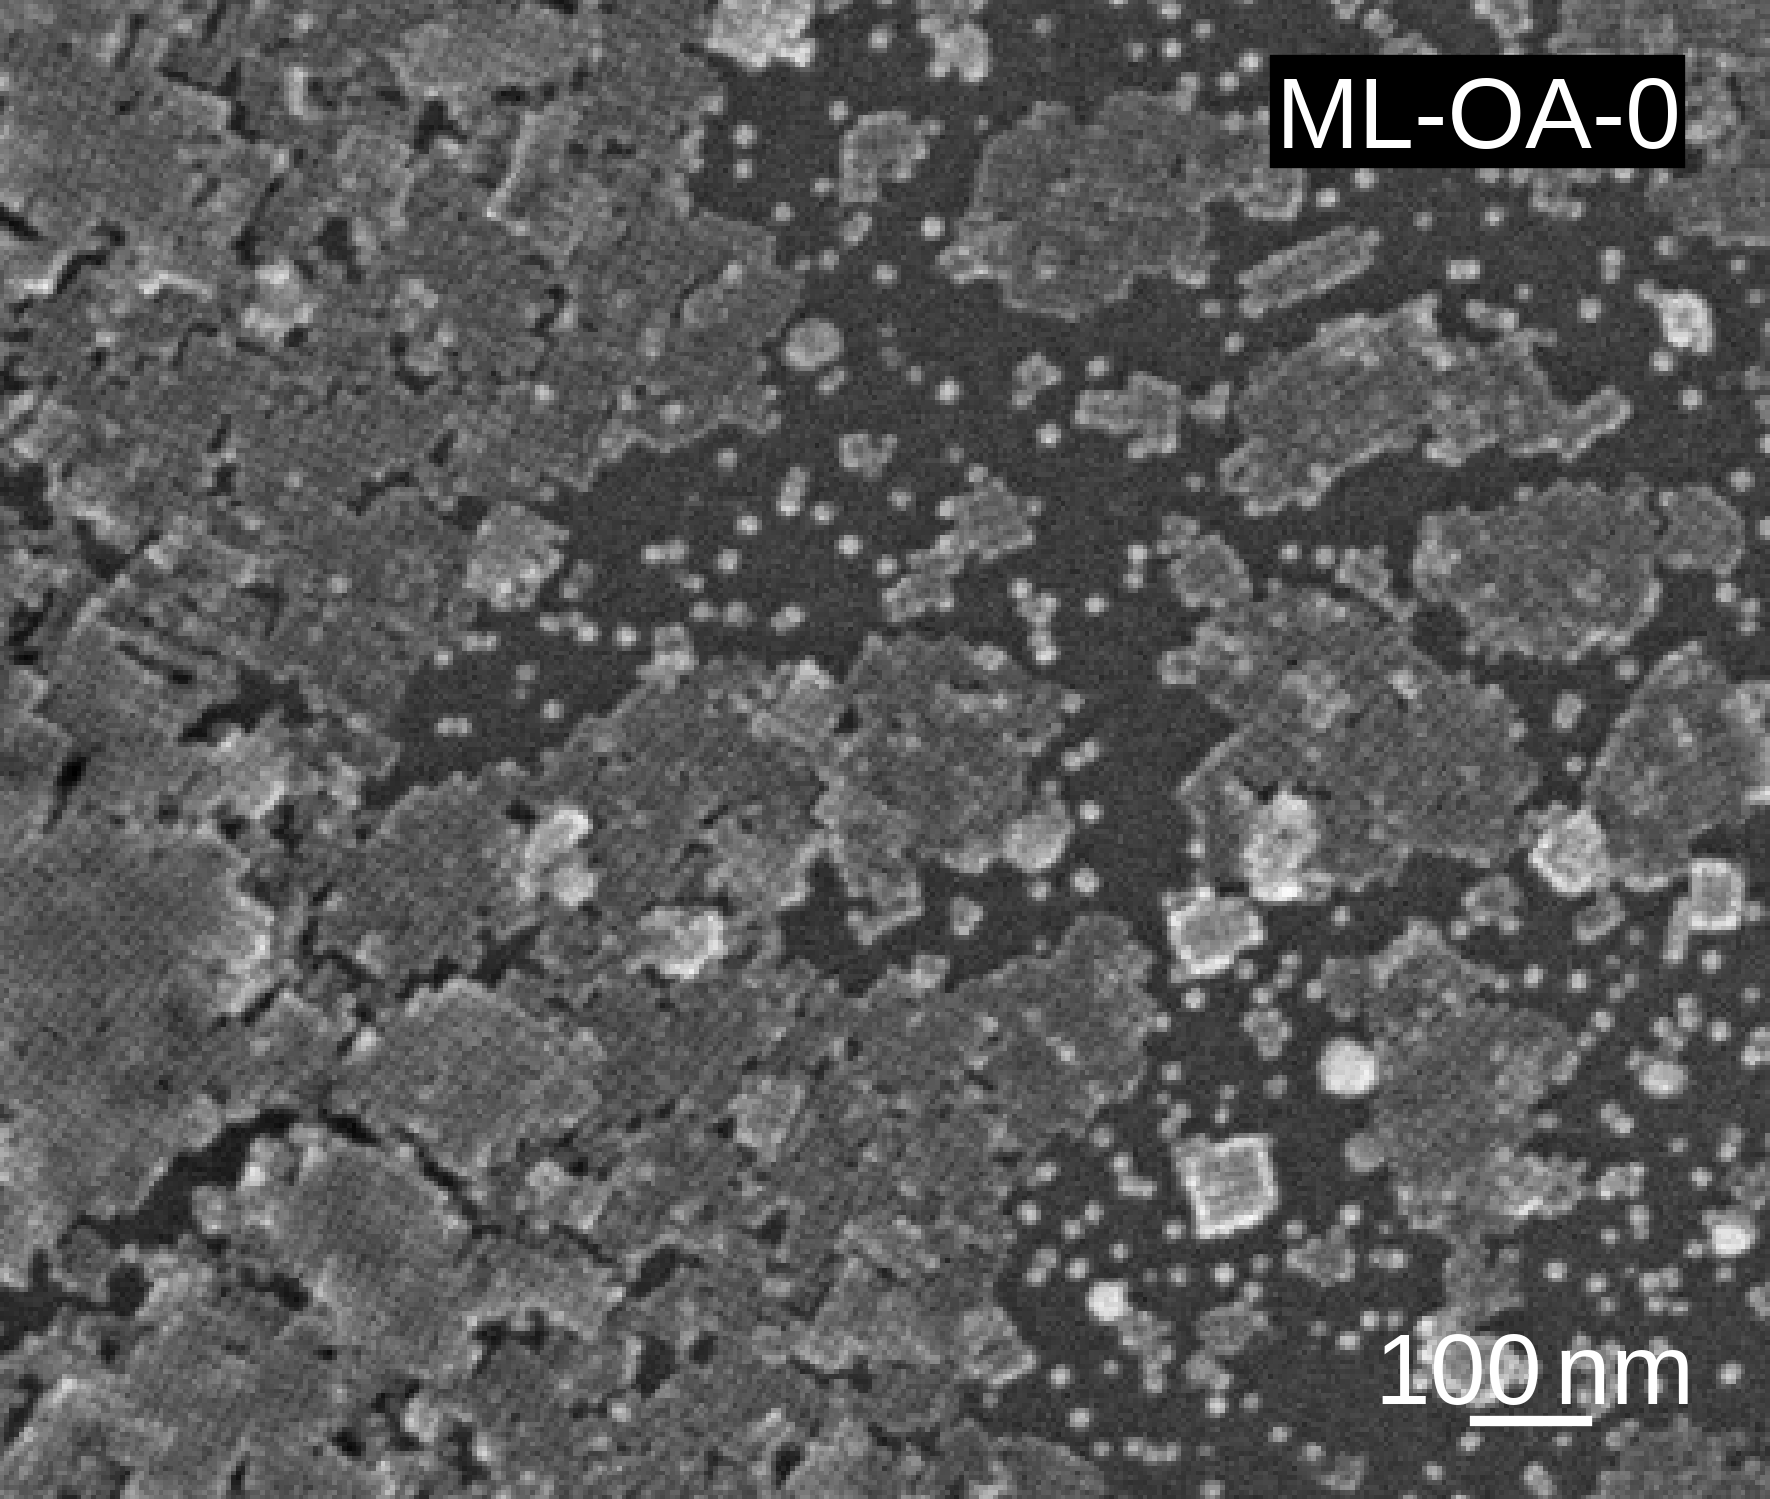
\includegraphics{monolayers_SEM_ML-OA-0}
    \caption{\label{fig:monolayers:preparation:solventVariation:NoOAAddend}SEM micrograph of Ac-CoFe-C-3 drop casted from a \textit{n}-heptane/octadecene dispersion.}
  \end{figure}

  Additionally to the alkene addend that is added, the fraction of oleic acid in the dispersion plays a role in the self-assembly process.
  Oleic acid is naturally in the dispersion from the synthesis procedure as became visible in the SANS characterization of the dispersions in \refsec{sec:monolayers:nanoparticle:sas}.
  From \reffig{fig:monolayers:preparation:solventVariation:NoOAAddend}, it is visible that drop casting Ac-CoFe-C-3 in a similar combination of \textit{n}-heptane/octadecene as discussed in the previous section shows no long range order formation.
  Instead disconnected sheets of short-range ordered nanocubes are visible across the substrate and single nanocubes are sprinkled around them.
  To discuss which influence the oleic acid content has on the long range order formation, four dispersions from the same stock solution and only varied oleic acid content are shown in \reffig{fig:monolayers:preparation:solventVariation:OAAddend}.

  \begin{figure}[tb]
    \centering
    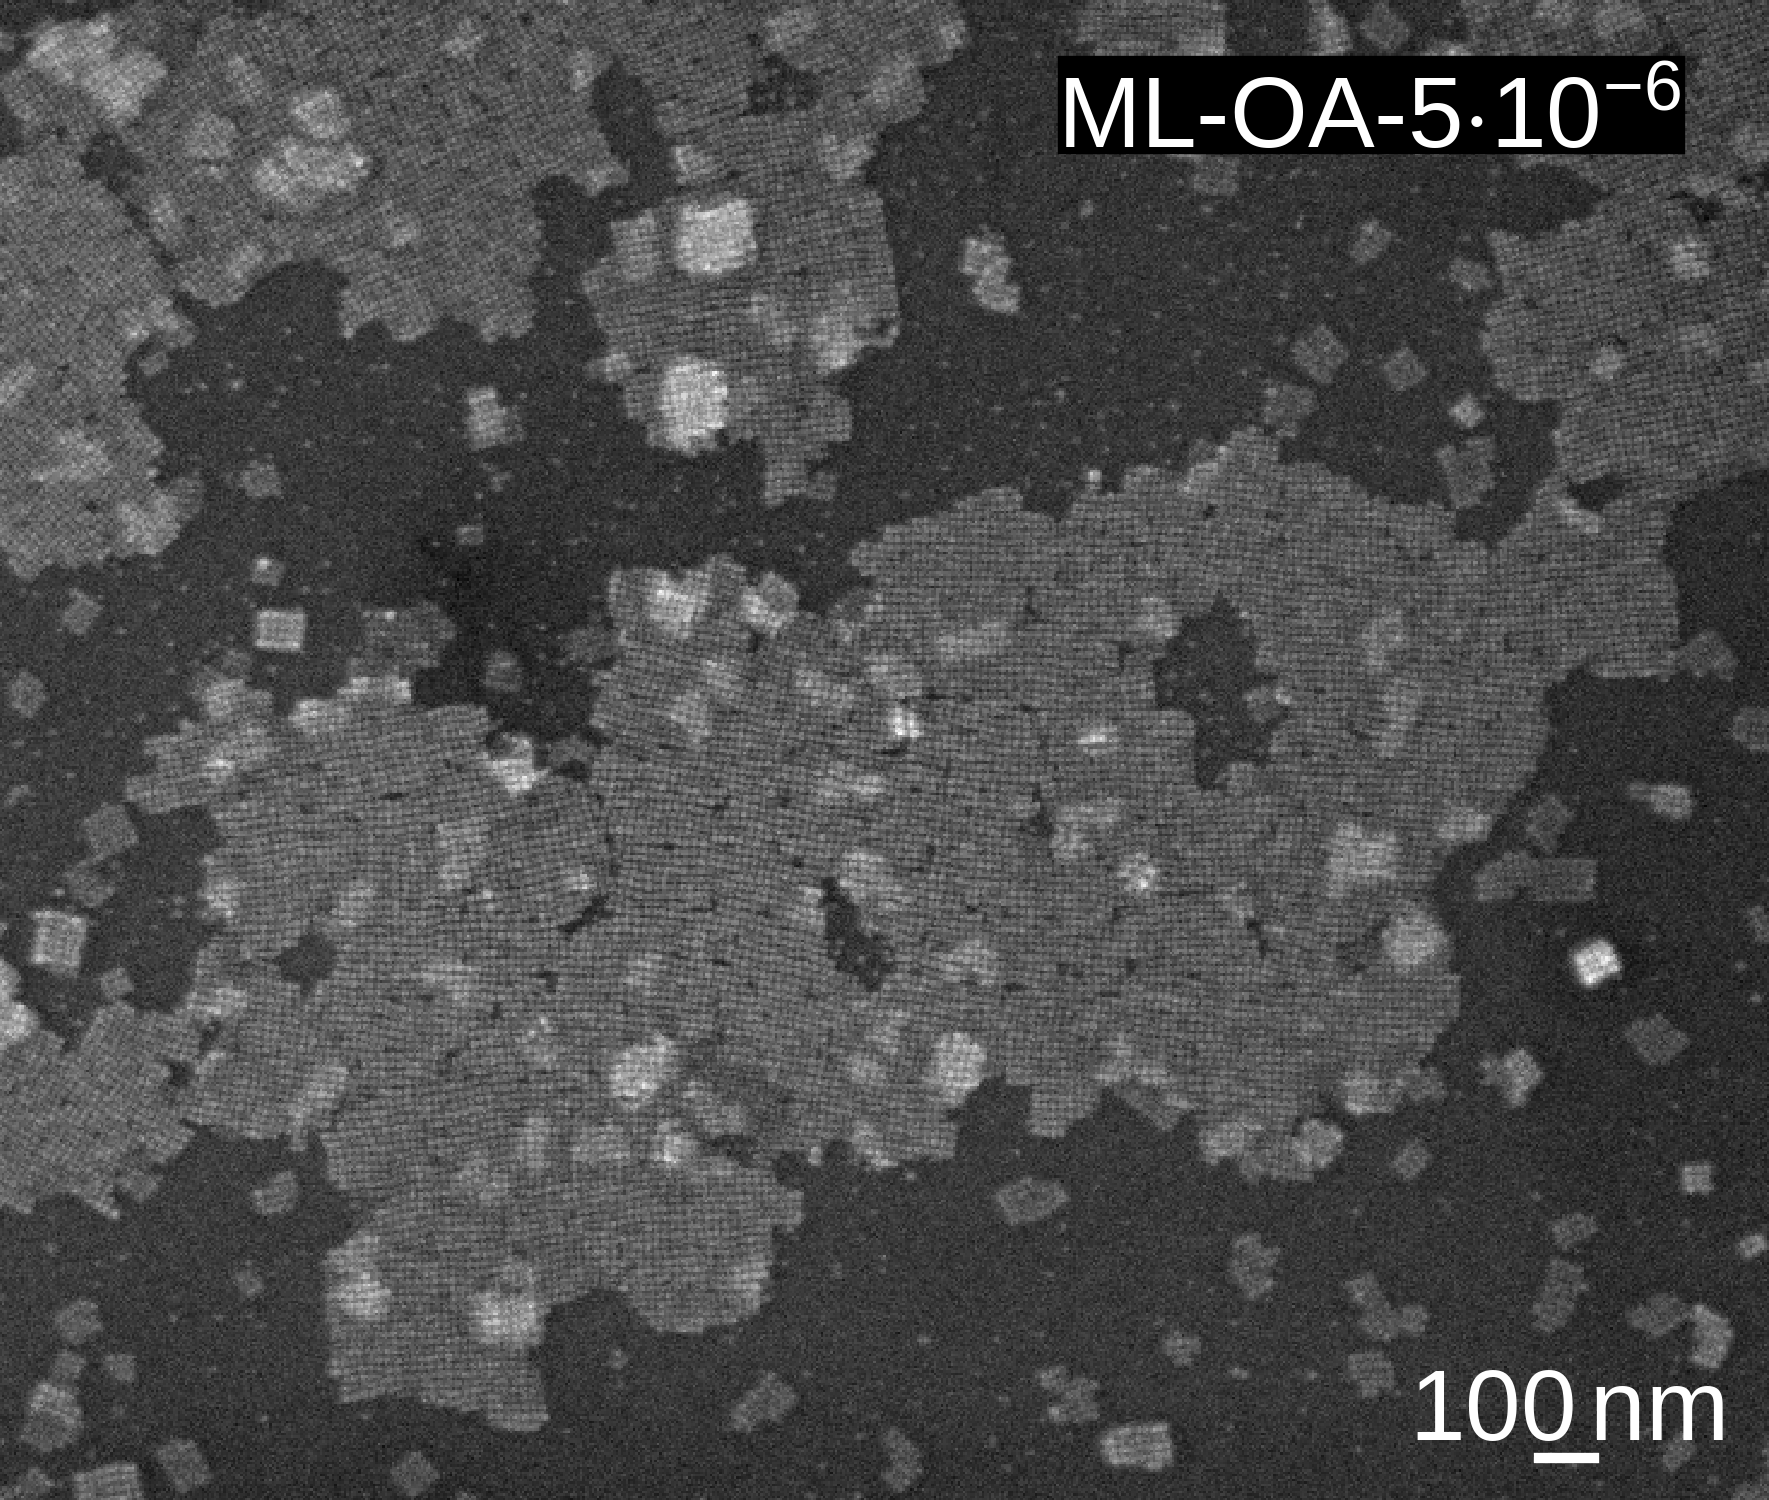
\includegraphics{monolayers_SEM_ML-OA-5e-6}
    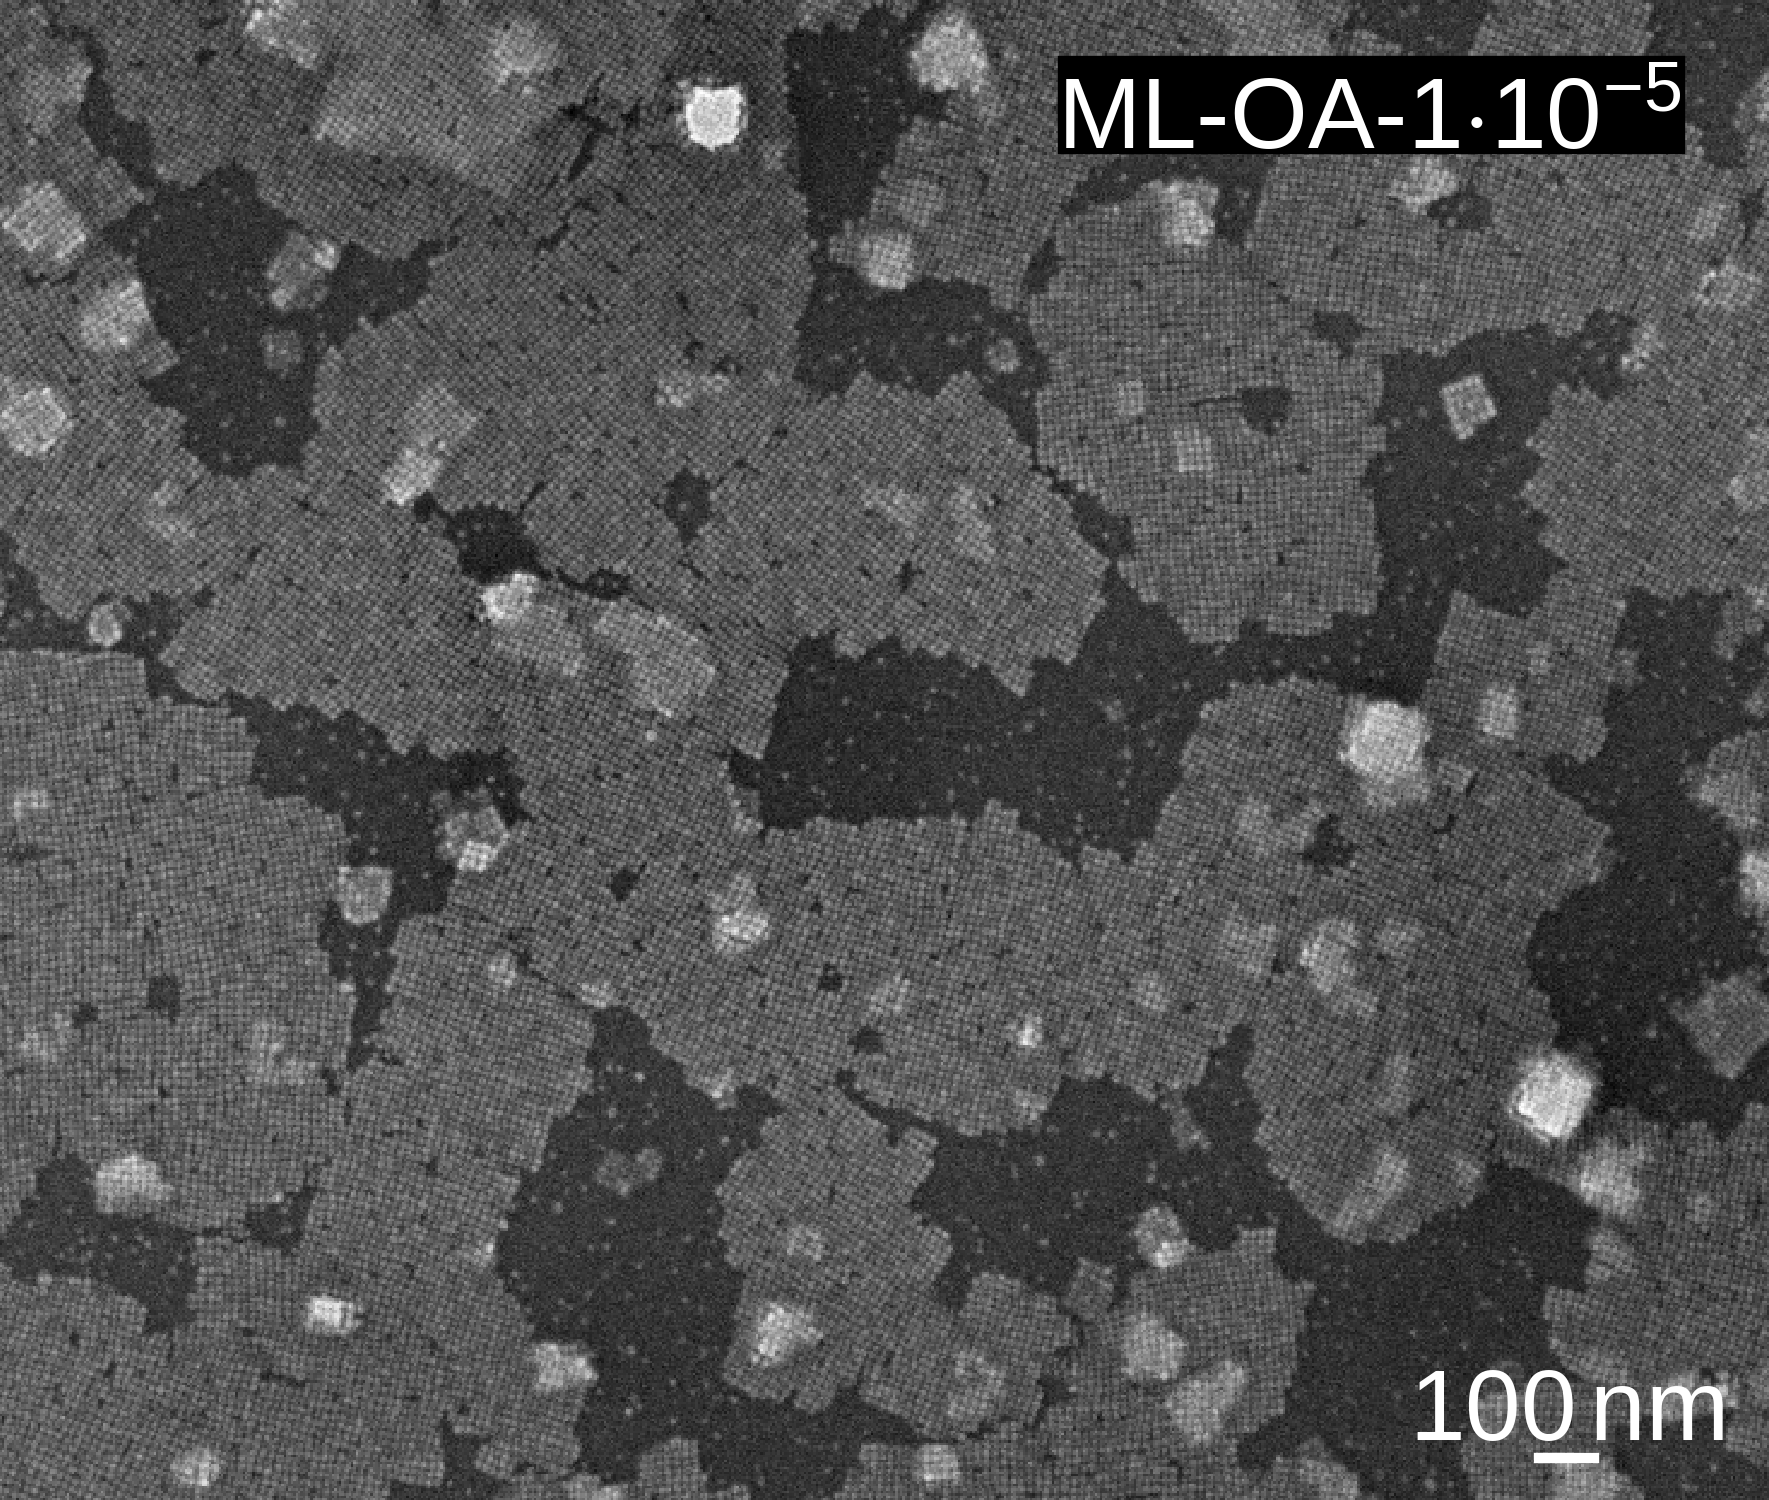
\includegraphics{monolayers_SEM_ML-OA-1e-5}
    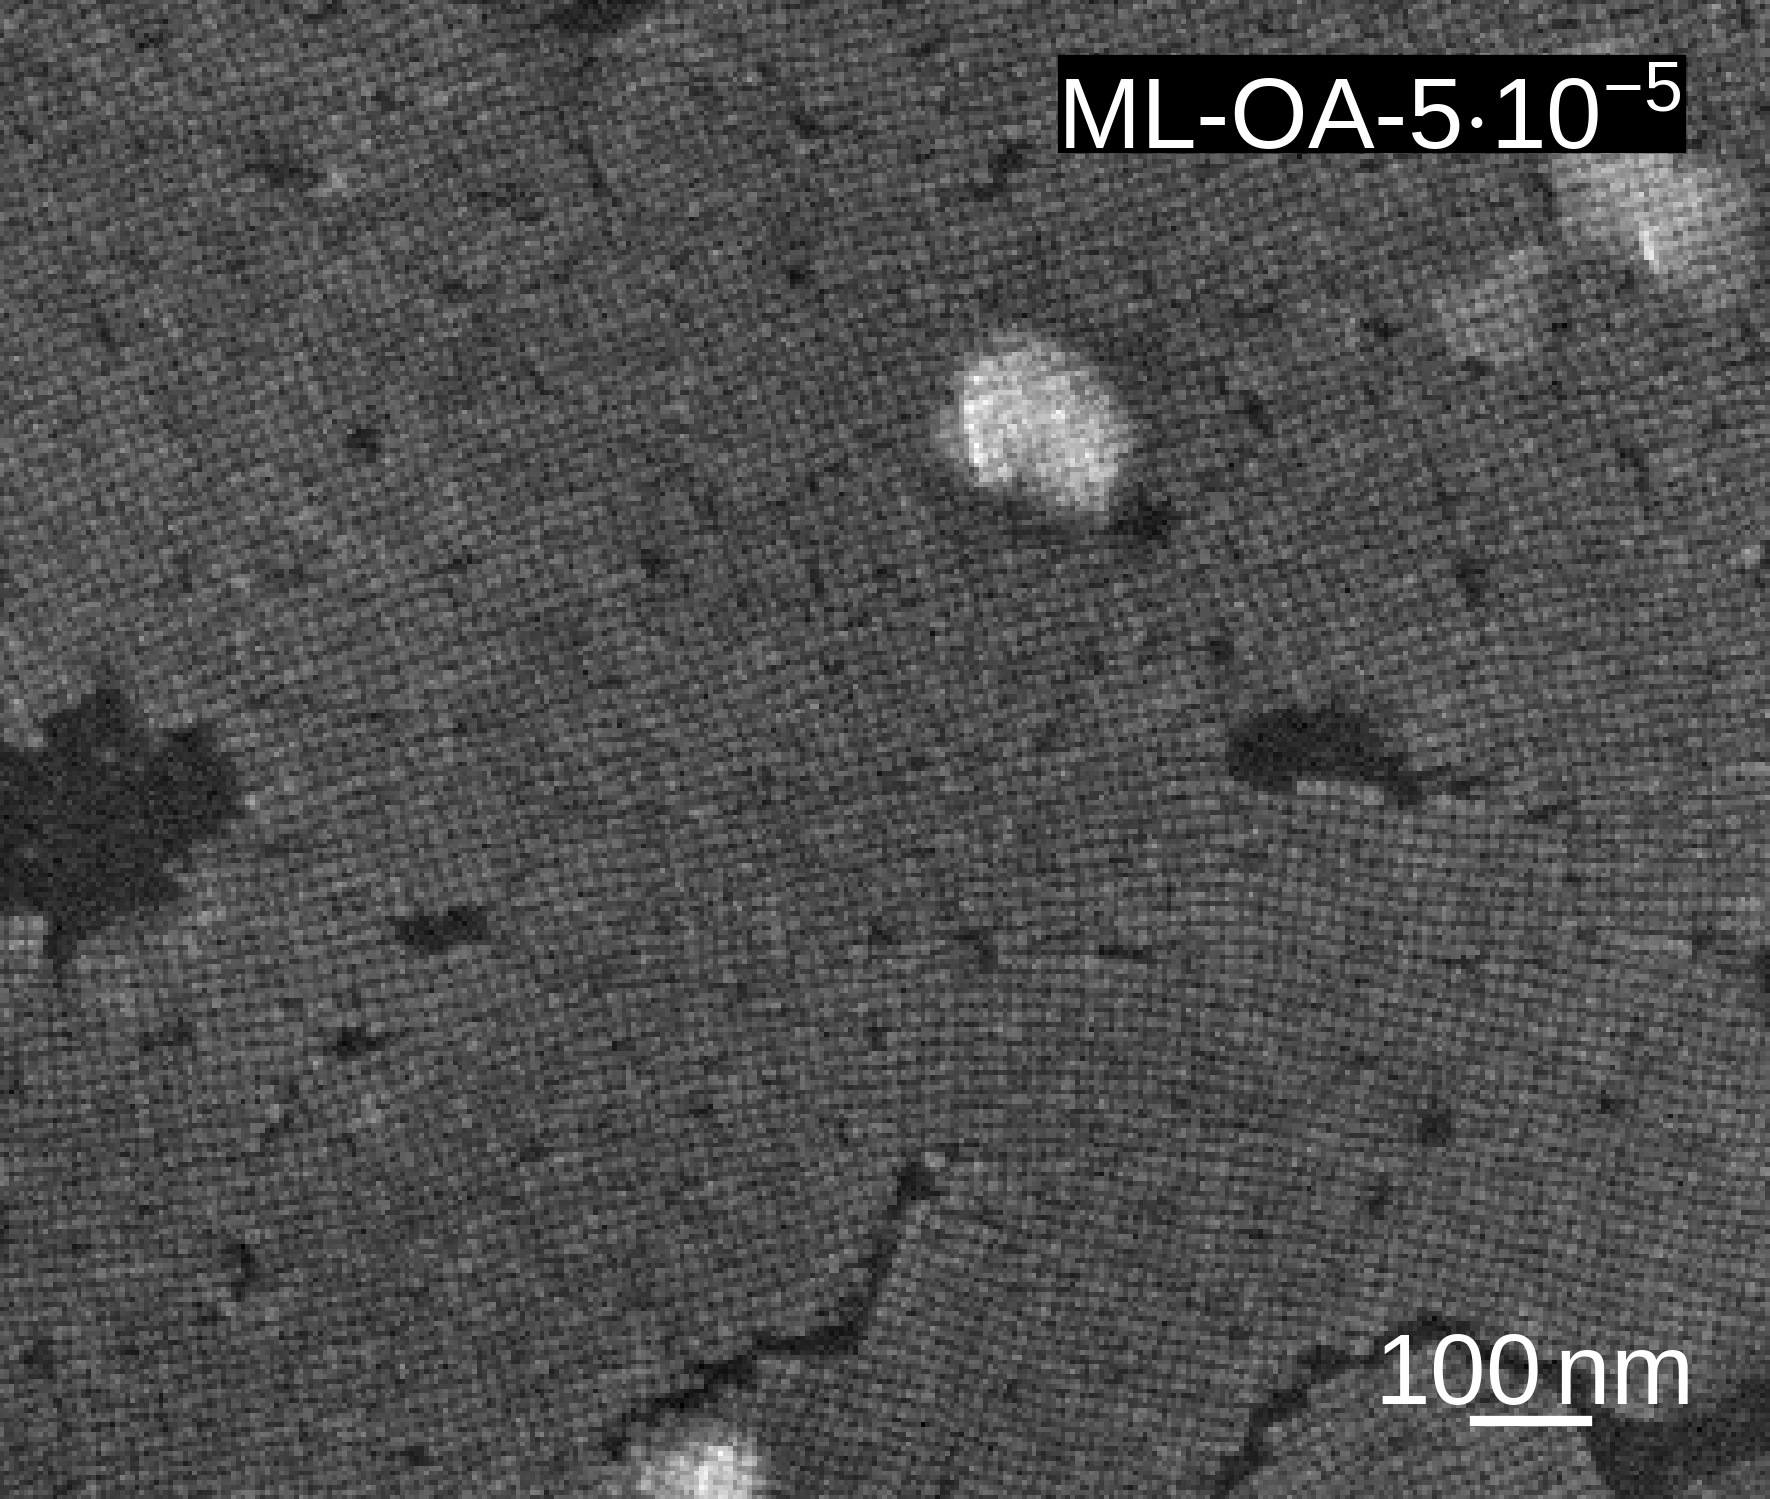
\includegraphics{monolayers_SEM_ML-OA-5e-5}
    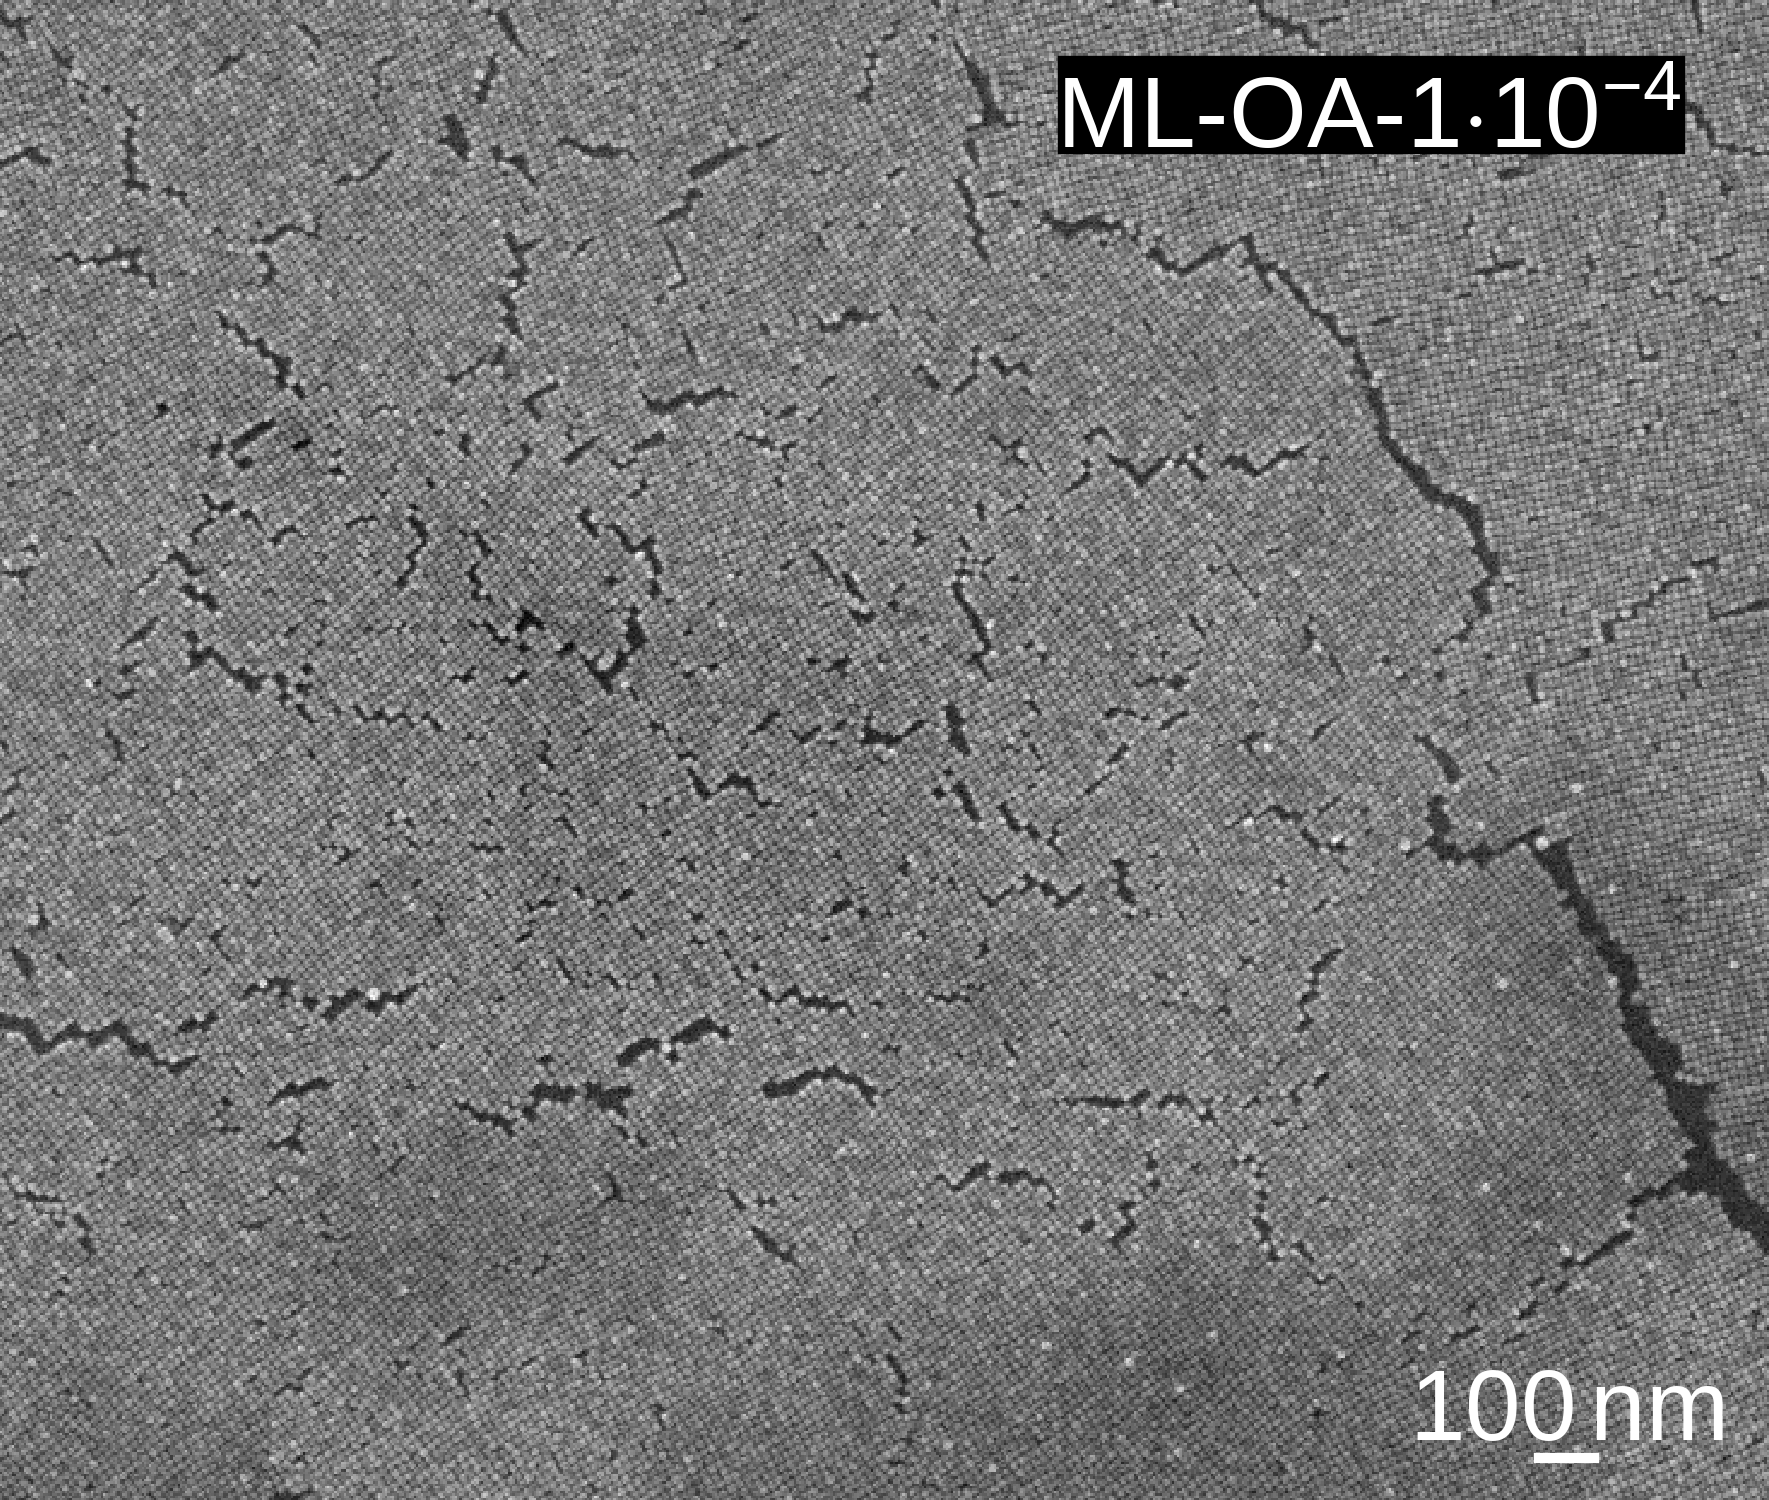
\includegraphics{monolayers_SEM_ML-OA-1e-4}
    \caption{\label{fig:monolayers:preparation:solventVariation:OAAddend}Variation of the oleic acid content analyzed in scanning electron microscopy. Monolayers drop casted from a dispersion of Ac-CoFe-C-3 with $5\cdot10^{-4} \unit{\%}$ (upper left), $1\cdot10^{-3} \unit{\%}$ (upper right), $5\cdot10^{-3} \unit{\%}$ (lower left) and $1\cdot10^{-2} \unit{\%}$ (lower right) oleic acid addend are shown.}
  \end{figure}

  The micrographs clearly show the trend for increasing long-ranged order with increase of the oleic acid content above $c_V^\textsf{OA} \eq 5\cdot10^{-3} \unit{\%}$.
  This concentration corresponds to a oleic acid film thickness of approximately $25 \unit{nm}$ if distributed homogeneously on the substrate surface.
  This coincides close to the nanocube size of approximately $12.5 \unit{nm}$.
  One is limited in the amount of oleic acid that can be add to the dispersion, as oleic acid as a high-boiling solvent is difficult to remove from the wafer after the drying of the primary solvent.
  It is reasonable to assume that the additional oleic acid during the final drying stage functions as a thin mobilization layer on which the nanocubes can still move in two dimensions, rearrange and reduce the defects in the lattice.
\end{document}